This is the third day! Most of the regular paper presentation happen today.

\subsection{Poster display}
\label{section:poster}

\begin{figure}[!ht]
    \centering
    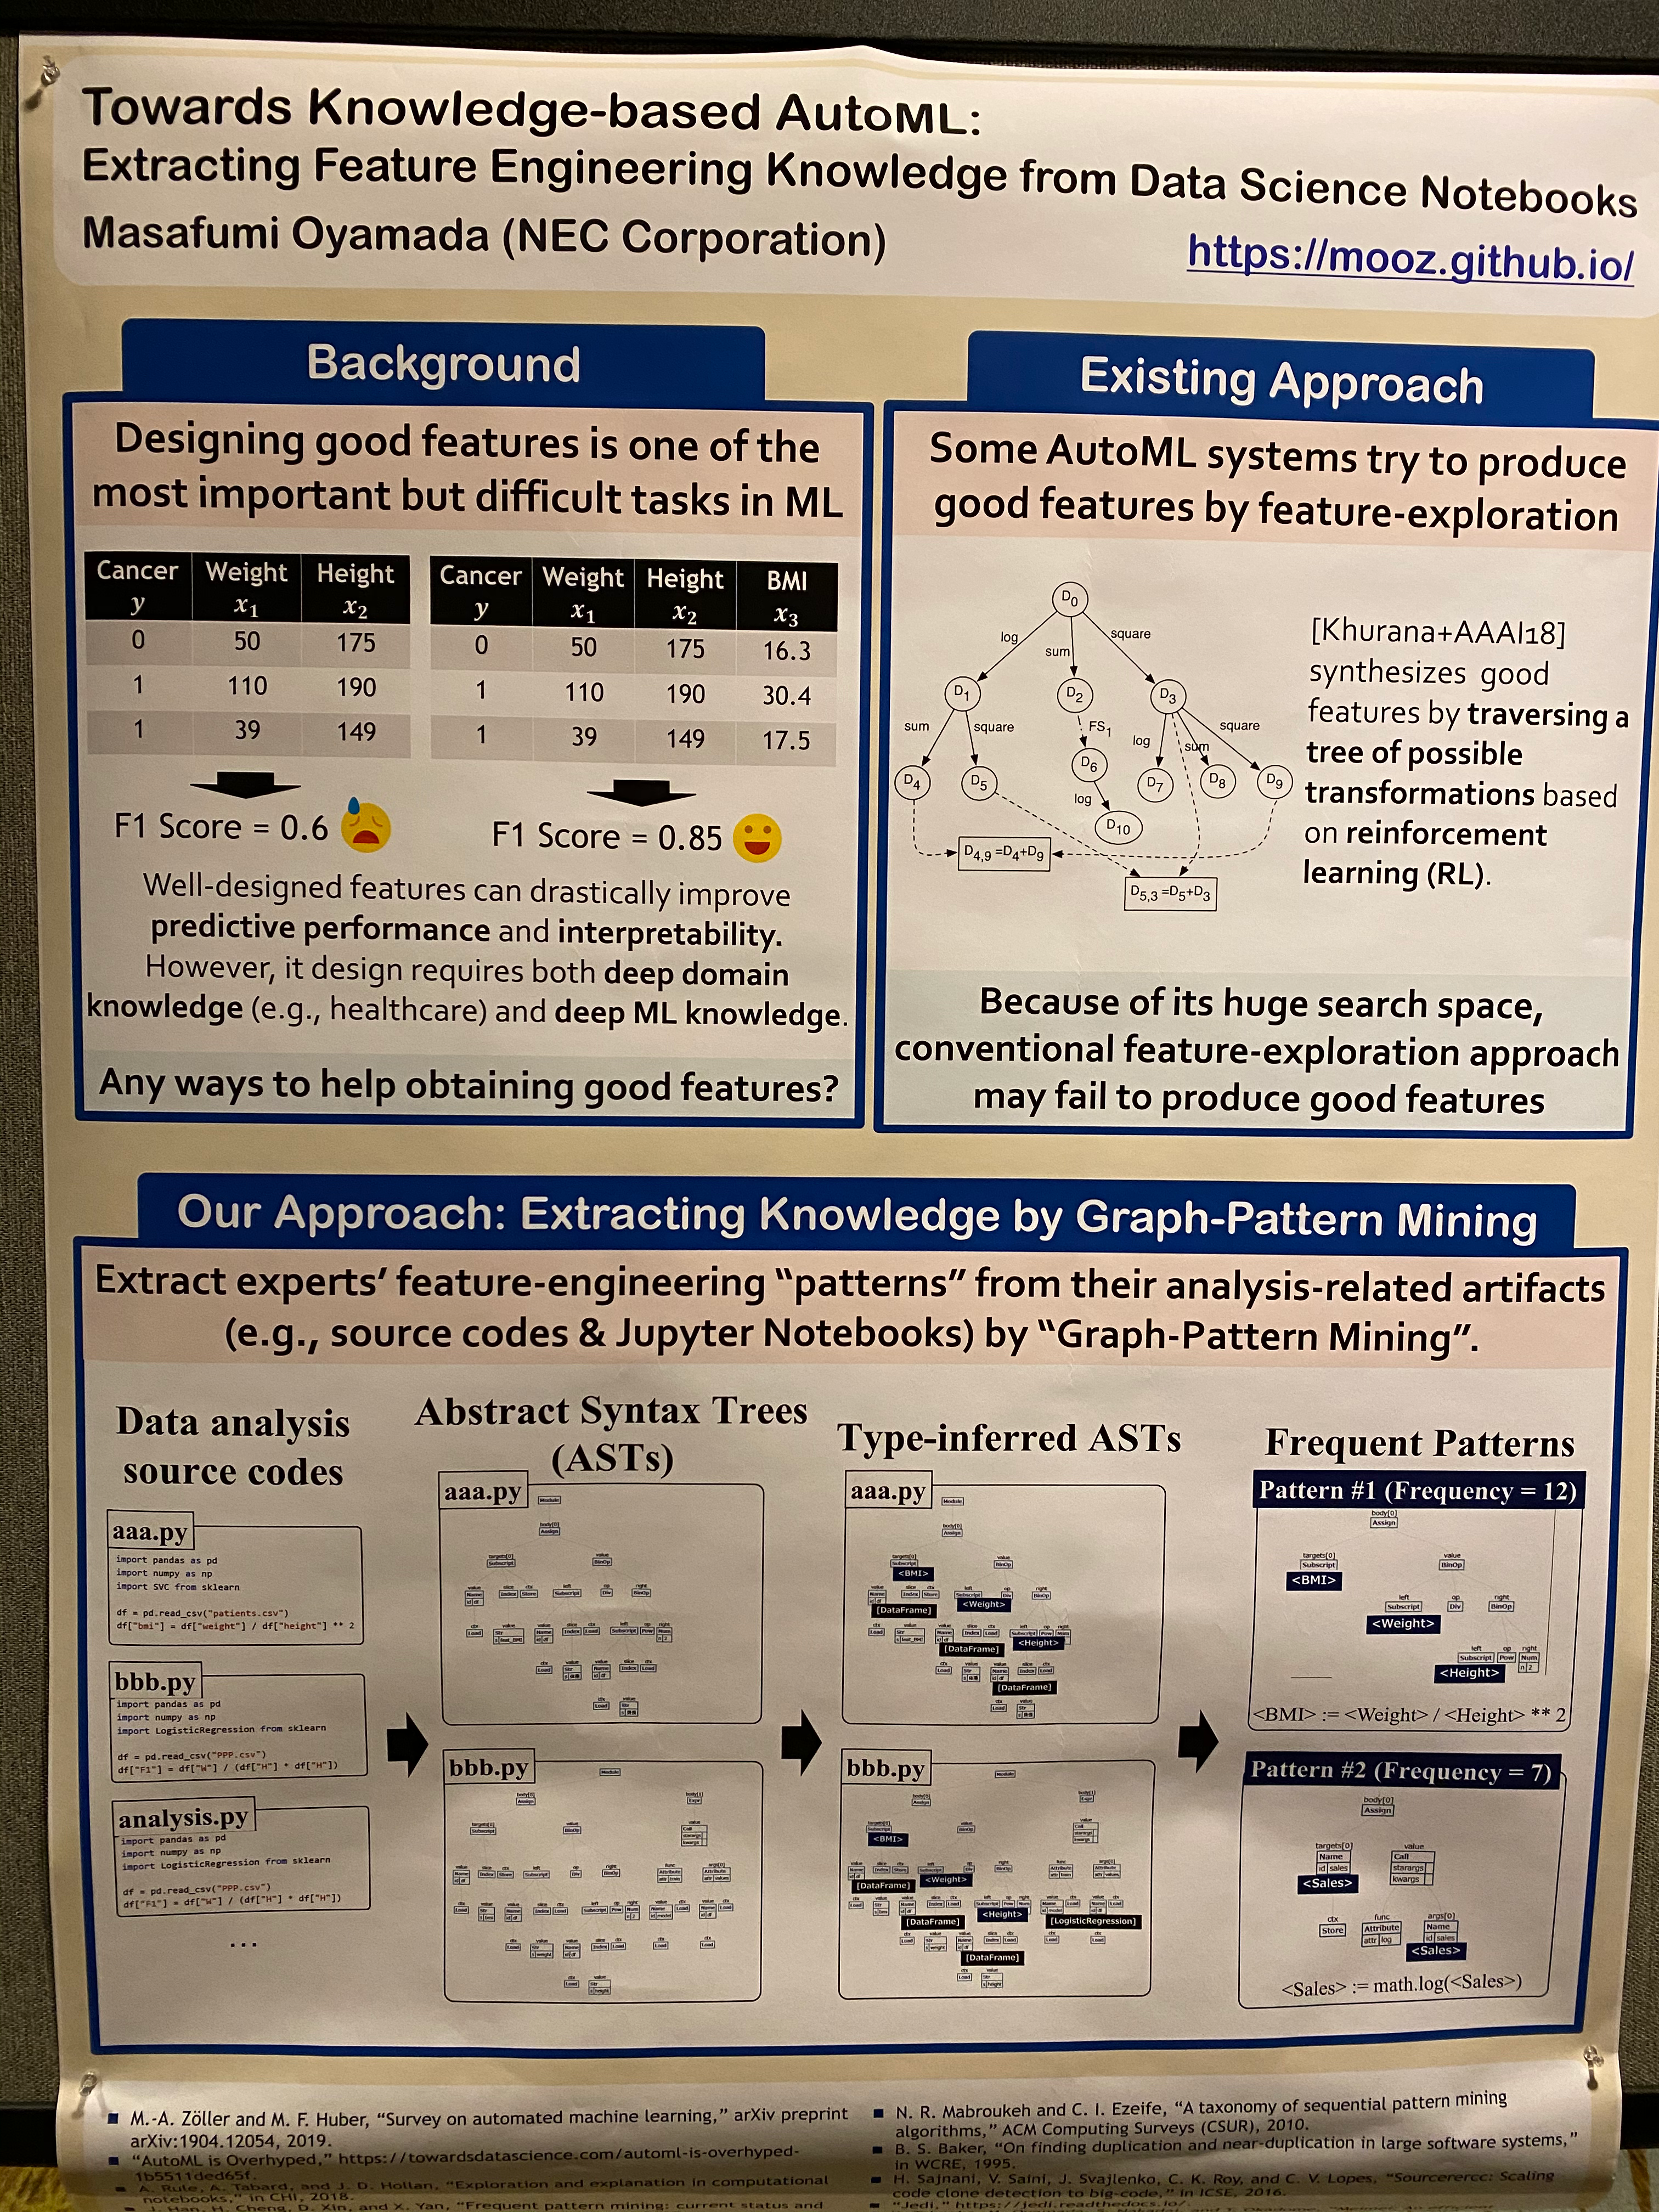
\includegraphics[width=120mm]{images/feature_engineering.png}
    \caption{Feature engineering with RL}
    \label{fig:my_label}
\end{figure}{}



\begin{figure}[!ht]
    \centering
    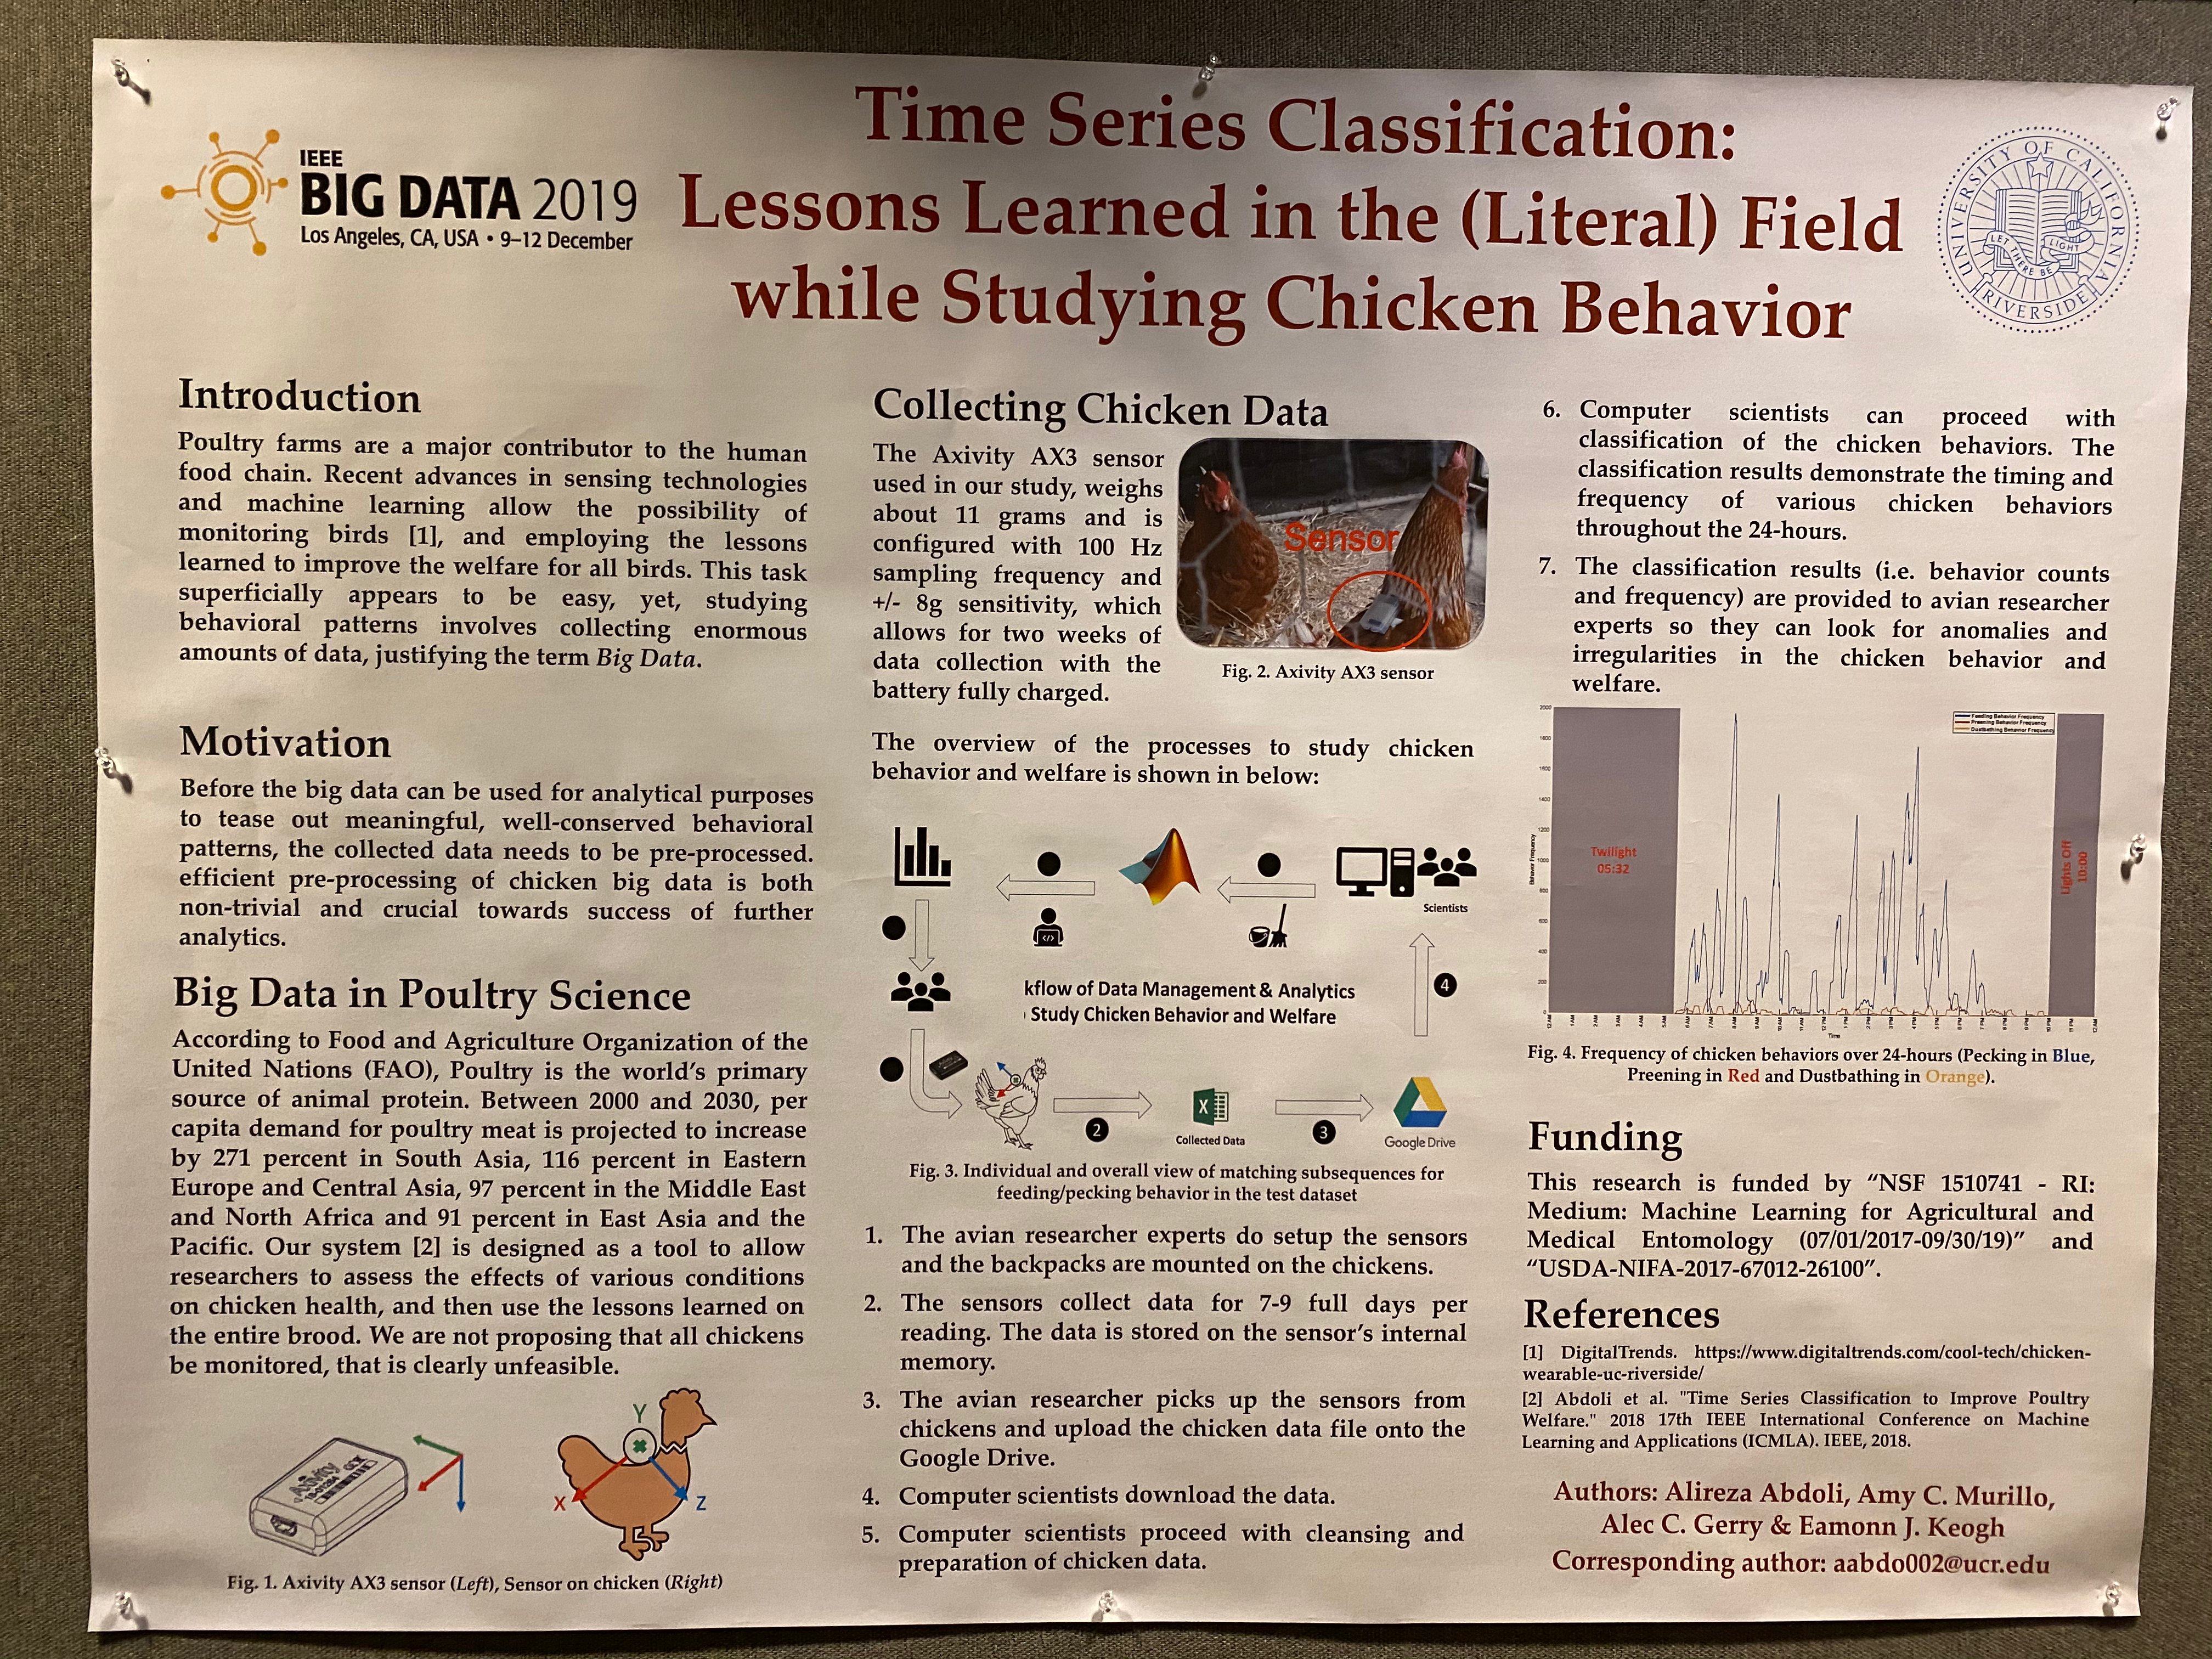
\includegraphics[width=120mm]{images/sarp_chicken.png}
    \caption{SARP on chicken?}
    \label{fig:my_label}
\end{figure}{}

\begin{figure}[!ht]
    \centering
    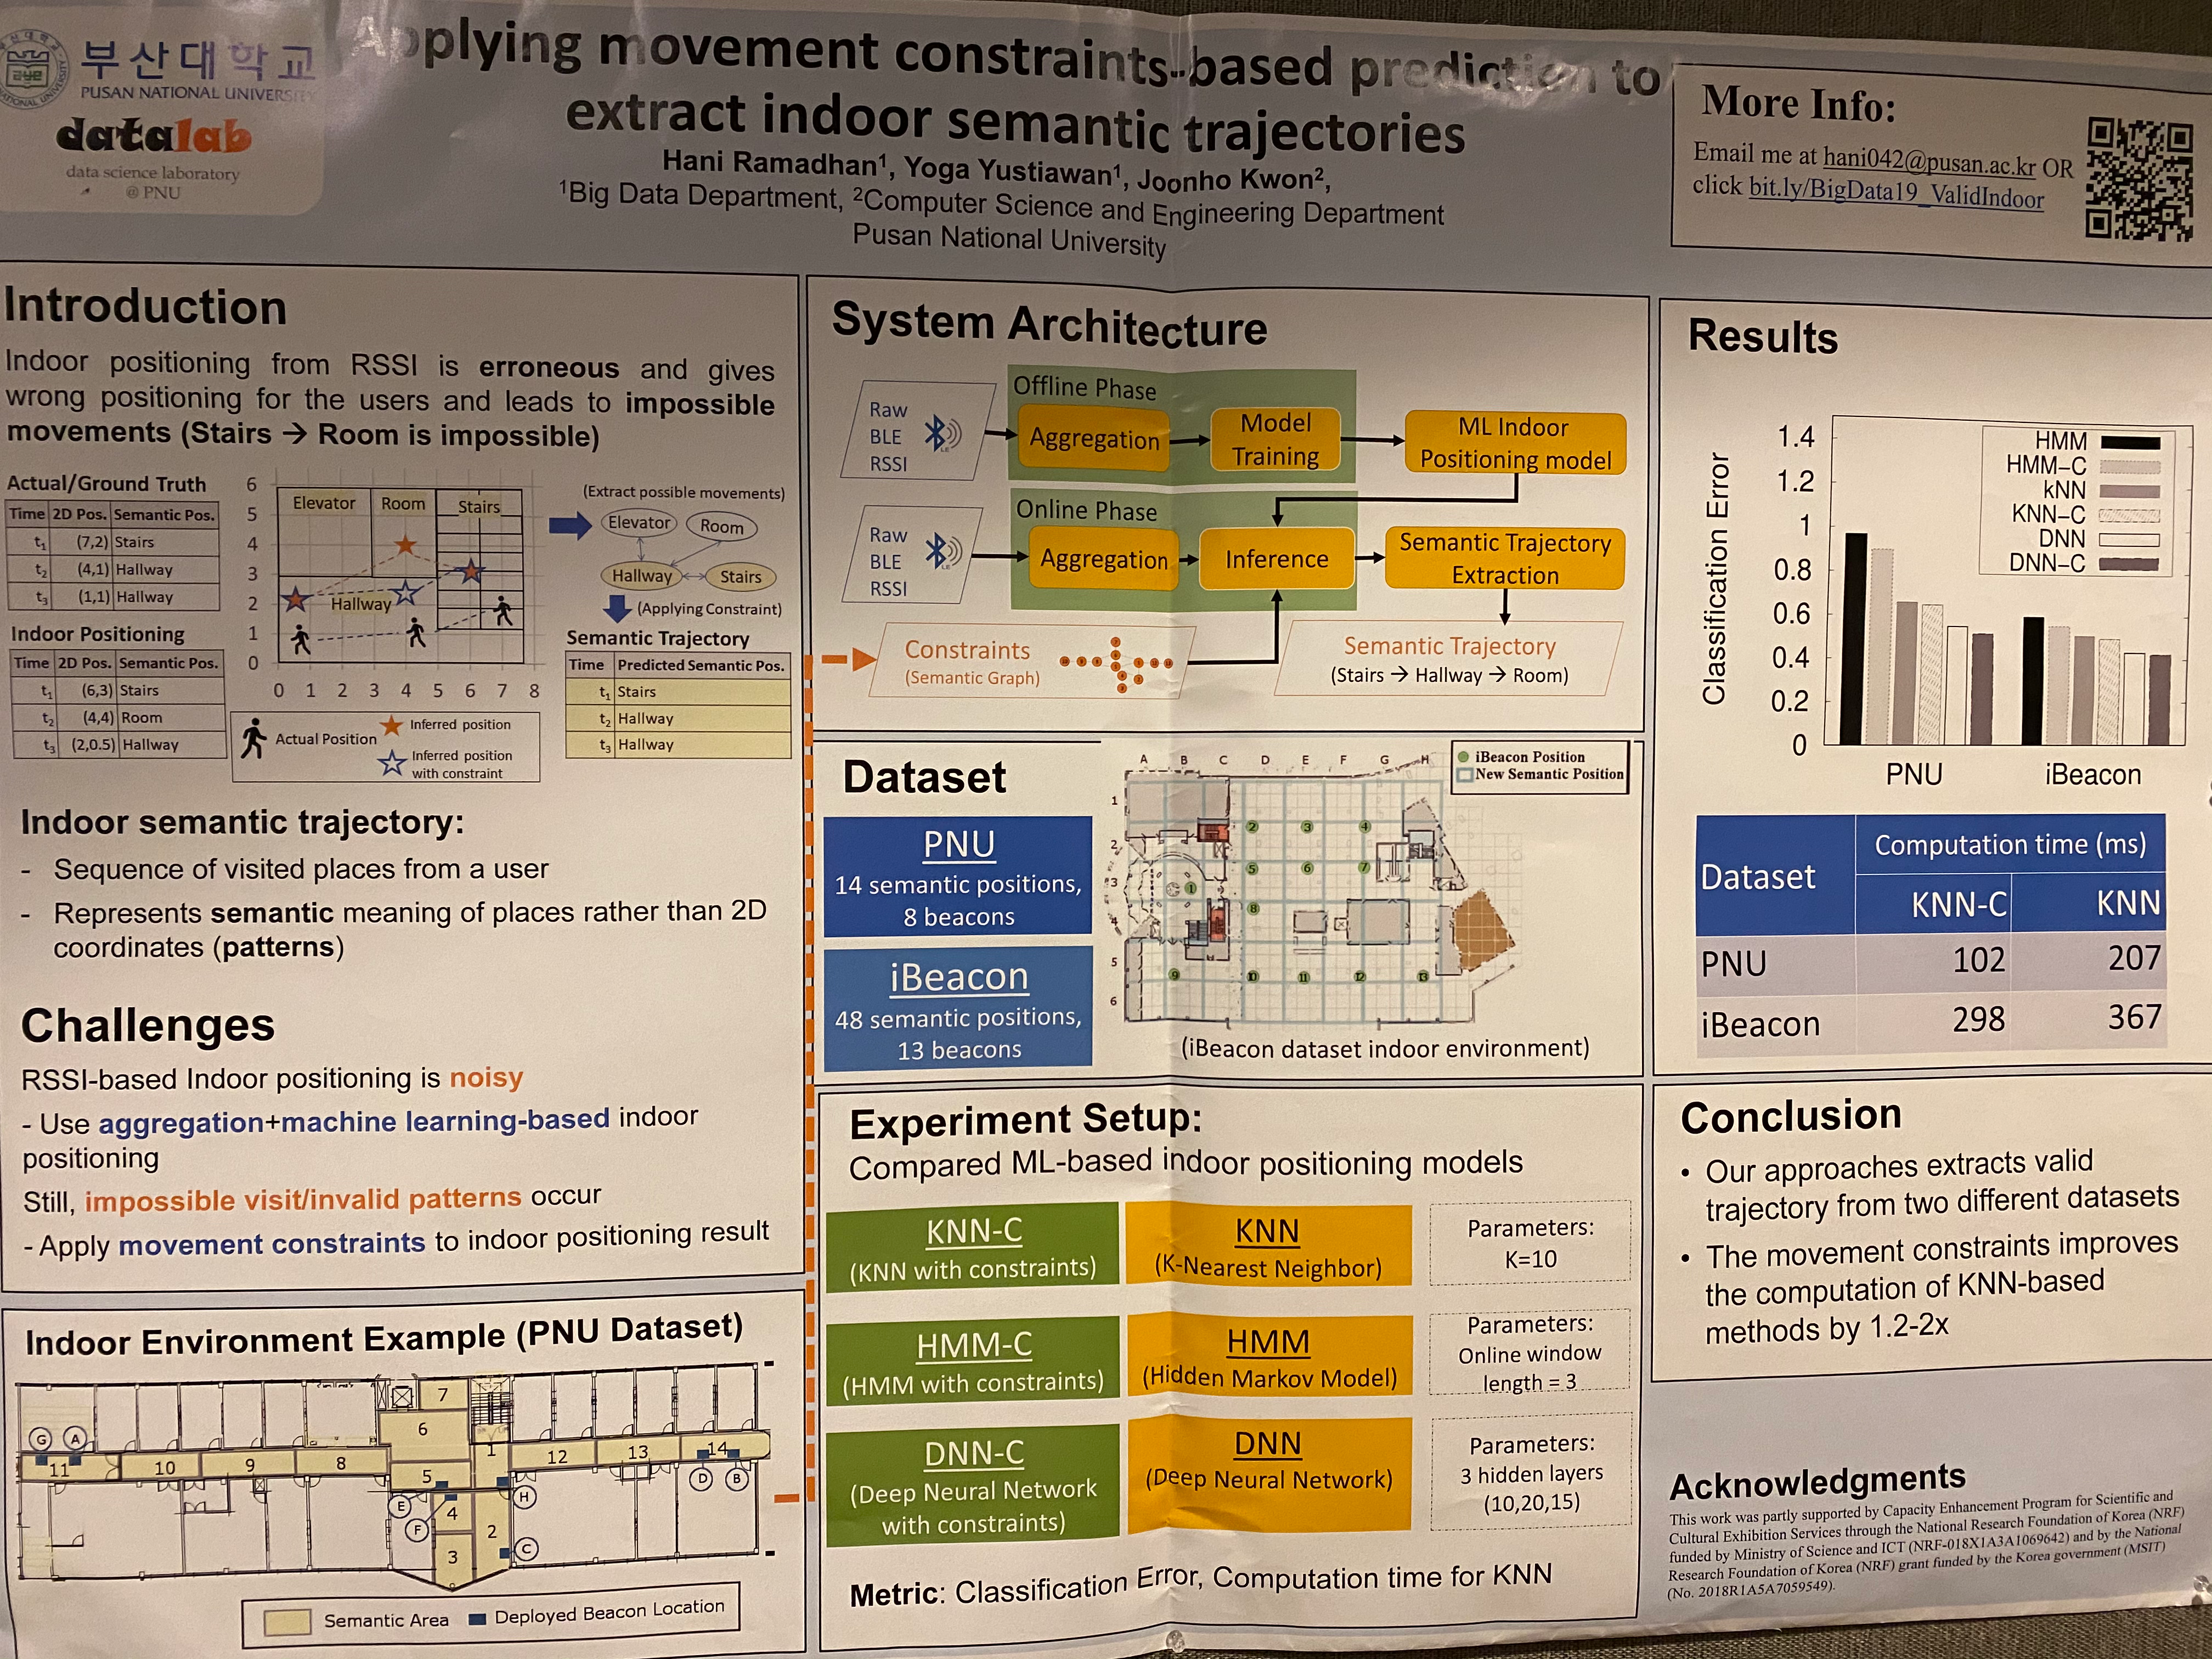
\includegraphics[width=120mm]{images/indoor.png}
    \caption{Indoor localization/trajectory prediction}
    \label{fig:my_label}
\end{figure}{}

\idea{Feature selection: using RL to do the feature selection, define a action graph where each feature is selected or not. then test the classifier on a small subset of the dataset. Then iterate the process.}

\idea{Causal discovery: similarly, can I use RL to find the causality. By deleting or adding the causal relations between the variables.}

\subsection{Complex Big Data Applications}

\idea{Multitask learning: can we apply MTL in FPG and Cardinal dataset?}

\subsection{New Computational Models for Big Data}

\subsubsection{Activation ensembles deep neural network}

$y_i=\sum_{i}\alpha_ih_i(\vec{x})$ where $h_i(\vec{x})$ is the activation function here (e.g., relu, tanh, etc.), and $\alpha$ is trainable. 

The optimization problem is defined as:

$$
minimize: \frac{1}{2}\sum(\hat{\alpha} - \alpha)^2
$$

$$
subject\ to: \sum_{n}\alpha_i = 1; \alpha_i \leq 0
$$

The results show that improvements are small but consistent in all experiments.

\subsubsection{Online federated learning}

For distributed data that are subject to privacy or security where data centralization is not possible.\\

$\ra$ Traditional approach: users' data from end device to central database\\
$\ra$ Proposed approach: models are built on end devices and the training parameters are transferred to central server. \\

\note{iPhone probably is deployed with this technology when learning ml models}

Federated multitask learning: each mobile device is considered as a separate task. \\

Federated multitask learning is formulated as an optimization problem:

\begin{figure}
    \centering
    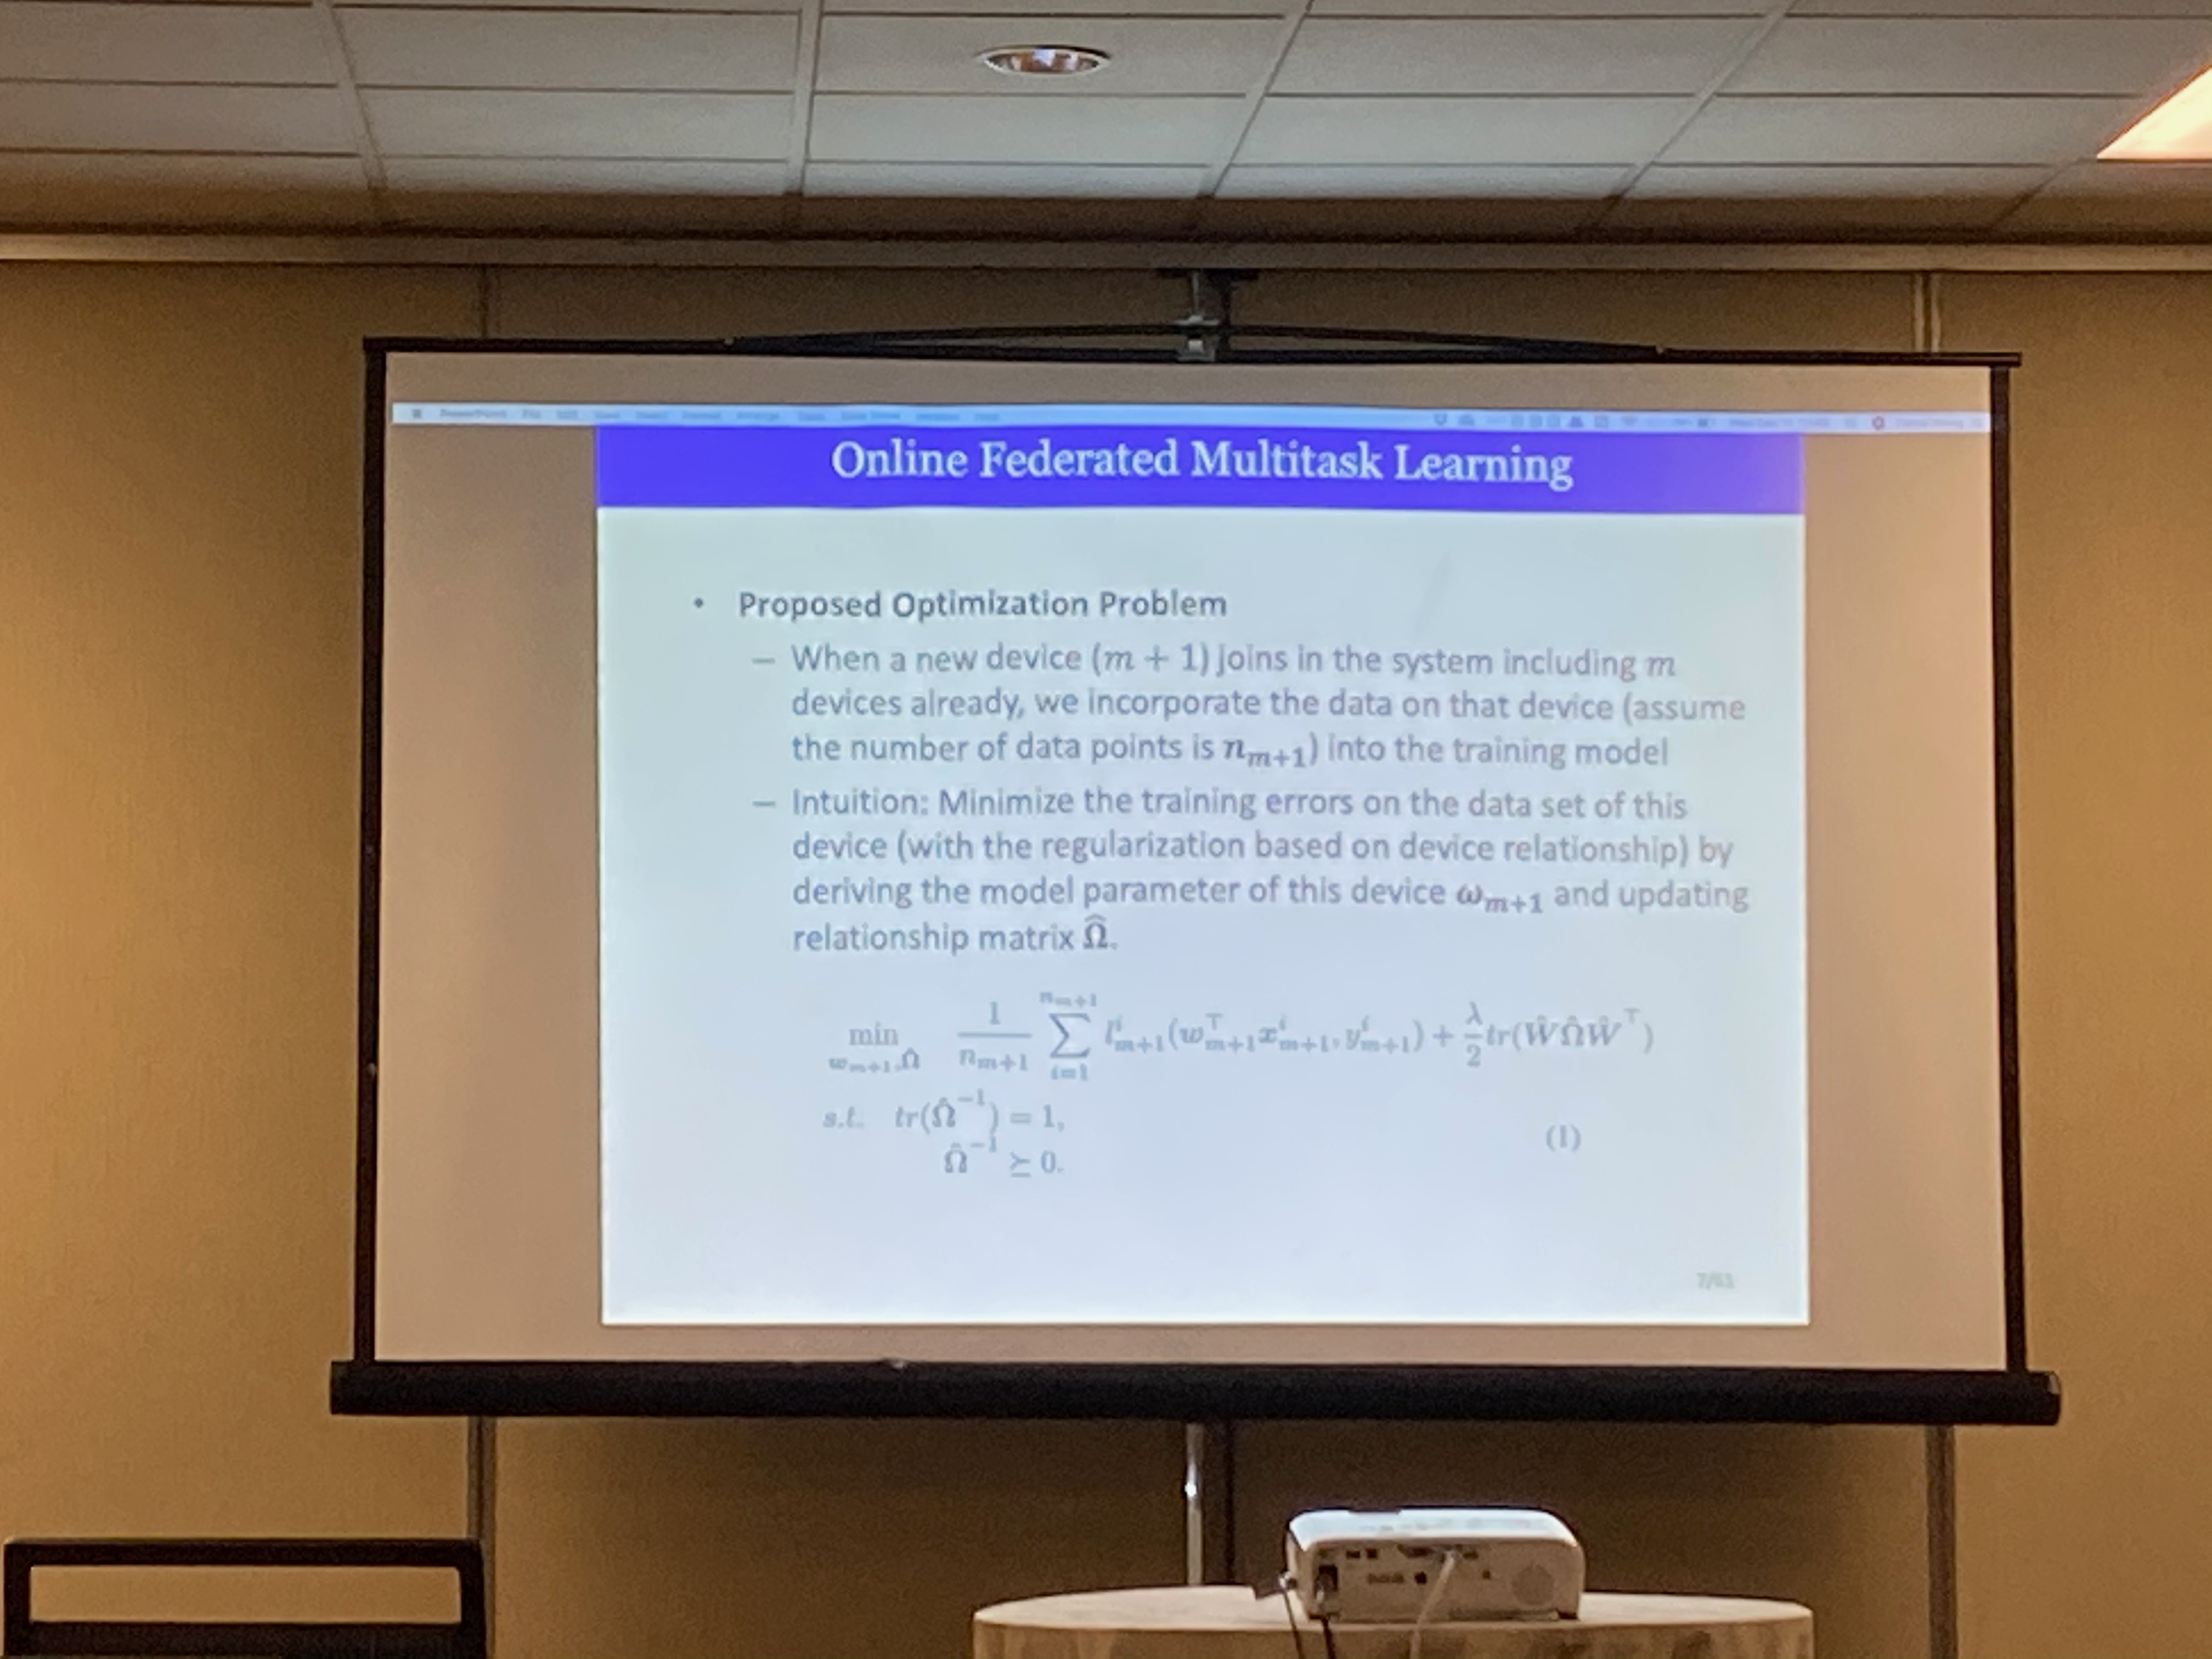
\includegraphics[width=120mm]{images/online_federated.png}
    \caption{Online federated as an optimization problem}
    \label{fig:my_label}
\end{figure}{}

{\bf Datasets}:

\begin{itemize}
    \item Human Activity Recognition 
    \item Eating Habit Monitoring
\end{itemize}{}



\subsection{Taming the complex unstructured data mining}

The speaker is Jiawei Han\footnote{\url{https://www.leiphone.com/news/201807/CWmEgpJaQmbHjkex.html}}.\\

$\ra$ Entity and relation extraction from text corpus. 

\idea{Can I  use entities and  relation extractions to mine causality relations in non-numeric dataset, such as text or images}

\spacerule

\subsection{Keynote: Data Commons}

\label{section:datacommmons}

The speaker is Guha from Google.\\

We have math equations models for areas that are simple but not for the domains that are complex.\\

Data Commons is a service where Google keeps a variety of datasets and provide open public access to them for data analytic. It's built with Python APIs. See \url{https://colab.research.google.com/drive/1qCPZZD0MPWx6CC34wFVJc_9B2-q0F-h_}\\

\remark{Basically, Data Commons is a better version of UCI machine learning repo.}

\note{Data journalism seems to be an interesting job}

\remark{\url{Schema.org} is a tool/service for extracting structured data from website and this might be very helpful in mining web/email information and creating datasets.}

\spacerule

\subsection{Panel: Addressing Big Data Heterogeneity: Recent Advances and Challenges}

\subsubsection{Big Data in the IoT Context}

{\bf TIPPERS Testbed: Testbed for IoT-based Privacy-Preserving PERvasive Spaces}

\subsubsection{Addressing Big Data Heterogeneity Challenges: Transforming Massive Unstructured Big Data into Structured Knowledge}

over 80\% data is unstructured data (e.g., text, media)

{\bf how to automatically generate structures from text data?}


\spacerule